\graphicspath{{img/chapter_1/}}

\chapter{Introduction}
\label{chapter:introduction}

\begin{synopsis}
Background on DM and its current status
\end{synopsis}
%%%%%%%%%%%%%%%%%%%%%%%%%%%%%%%%%%%%%
%%%%%%%%%%%%%%%%%%%%%%%%%%%%%%%%%%%%%
%%%%%%%%%%%%%%%%%%%%%%%%%%%%%%%%%%%%%

Dark Matter is an enigma in modern physics. Despite the significant scientific
effort that has gone into trying to discern its nature, a definitive detection
proving its existence eludes us. Nevertheless, dark matter's influence 
on our universe is undeniable, with evidence supporting its existence arising on \fixMV{all} scales, large and small.


%%%%%%%%%%%%%%%%%%%%%%%%%%%%%%%%%%%%%
%%%%%%%%%%%%%%%%%%%%%%%%%%%%%%%%%%%%%
%%%%%%%%%%%%%%%%%%%%%%%%%%%%%%%%%%%%%
\section{Evidence for Dark Matter}
%%%%%%%%%%%%%%%%%%%%%%%%%%%%%%%%%%%%%
%%%%%%%%%%%%%%%%%%%%%%%%%%%%%%%%%%%%%
%%%%%%%%%%%%%%%%%%%%%%%%%%%%%%%%%%%%%

Today, the amount of evidence in support of dark matter's existence is overwhelming. This evidence comes from astrophysical and cosmological observations that are inconsistent with a universe composed entirely of visible matter. This section serves as a review of this evidence. 

%%%%%%%%%%%%%%%%%%%%%%%%%%%%%%%%%%%%%
%%%%%%%%%%%%%%%%%%%%%%%%%%%%%%%%%%%%%
\subsection{Astrophysical Observations}
%%%%%%%%%%%%%%%%%%%%%%%%%%%%%%%%%%%%%
%%%%%%%%%%%%%%%%%%%%%%%%%%%%%%%%%%%%%

\subsubsection*{Galaxy Clusters}

Some of the first hints of dark matter's existence came from observations of galaxy clusters. Perhaps the most famous analysis was performed by Fritz Zwicky~\cite{Zwicky:1937zza_MassesNebulaeClusters}, who was puzzled by the high rotational velocities of galaxies within the Coma Cluster. By applying the virial theorem, equating the cluster's kinetic and gravitational potential energies, he found that the cluster would need to contain a much greater amount of \textit{dunkle materie} (dark matter) than visible matter in order to accommodate these high velocities.

\subsubsection*{Rotation Curves of Spiral Galaxies}

The anomalous rotational velocities observed in galaxy clusters can also be observed at the galactic scale. The rotation curves of spiral galaxies, which relate the rotational velocities of stars to their distance from the galactic centre, were observed to be flat at large distances. From the observed distribution of visible matter, Newtonian mechanics predicts that the orbital velocity of a star a distance $r$ from the galactic centre, $v_\star(r)$, is related to the mass of the galaxy, $M(r)$, through
\begin{equation}
    v_\star(r) = \sqrt{\frac{G M(r)}{r}},
\end{equation}
indicating that the velocity should fall off as $1/\sqrt{r}$ at the outer regions of the galaxy where $M(r)$ is constant. Instead, observations of many spiral galaxies indicate that this velocity remains constant out to the edge of the galaxy. 

A simple way to produce such a rotation curve is to introduce a spherically symmetric distribution of dark matter around the galaxy,
\begin{equation}
    \rho_{\mathrm{DM}}(r) = \frac{v_0^2}{4 \pi G r^2},
\end{equation}
that results in a constant rotational velocity of $v_0$ all the way out to the galaxy edge. Detailed simulations of structure formation in a Cold Dark Matter (CDM) universe indicate that the dark matter halo follows a Navaro-Frenk-White (NFW) profile, \fixMV{cite for NFW}
\begin{equation}
    \rho_{\mathrm{DM}}(r) = \frac{\rho_0}{\left( \frac{r}{r_\mathrm{s}}\right)\left( 1 + \frac{r}{r_\mathrm{s}}\right)^2},
\end{equation}
where $\rho_0$ and $r_\mathrm{s}$ are free parameters that must be fit to each individual halo. 
% More detailed simulations show that the true profile deviates slightly from an NFW, instead being more appropriately modeled by an Einasto profile. However, both profiles are observationally indistinguishable.

An example rotation curve for galaxy NGC 6503 is presented in Fig.~\ref{fig:gal_rotn_curve}, with the contributions from each of the matter components to the rotational velocity shown~\cite{Freese:2008cz_may_ReviewObservationalEvidence, Lelli:2016zqa_SPARCMassModels}. As can be seen, the visible matter constituting disk and gas components do not explain the observed rotational velocity. 

\begin{figure}[t!]
    \centering
    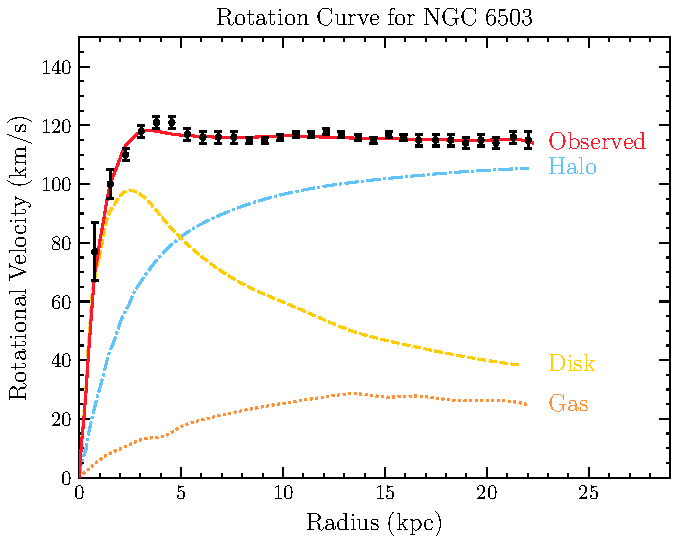
\includegraphics{gal_rotn_N6503.pdf}
    \caption{Galaxy rotation curve for NGC 6503, showing the contributions to the total velocity (red) from the DM halo (blue), disk (yellow), and gas components. Data used in making this plot was obtained from~\cite{Freese:2008cz_may_ReviewObservationalEvidence, Lelli:2016zqa_SPARCMassModels}.}
    \label{fig:gal_rotn_curve}
\end{figure}

\subsubsection*{Gravitational Lensing}

As described by General Relativity, the curvature of space-time around massive entities causes light to travel along curved paths. As such, the mass of astrophysical structures can be deduced from the extent to which objects in the background are gravitationally lensed. The disparity between the mass obtained from gravitational lensing and the mass of visible matter in the system is further evidence of dark matter's existence. 

\subsubsection*{The Bullet Cluster}

The bullet cluster is the result of two colliding galaxy clusters which the Chandra X-ray telescope imaged. When viewed in the X-ray, the smearing of the visible matter after the collision is clearly seen, as shown in the red regions of Fig.~\ref{fig:bullet_cluster}, which is expected from such a collision. However, when the gravitational potential was mapped using gravitational lensing, it was clear that the majority of the mass was displaced relative to the visible matter. This mass is attributed to the dark matter components of the original clusters. As indicated by the purple regions in Fig.~\ref{fig:bullet_cluster}, the dark matter halos seem to have passed through each other mostly unperturbed. This tells us that not only is the majority of the mass comprised of dark matter, but that the dark matter has extremely small interactions with both the visible matter and itself. 

\begin{figure}[t!]
    \centering
    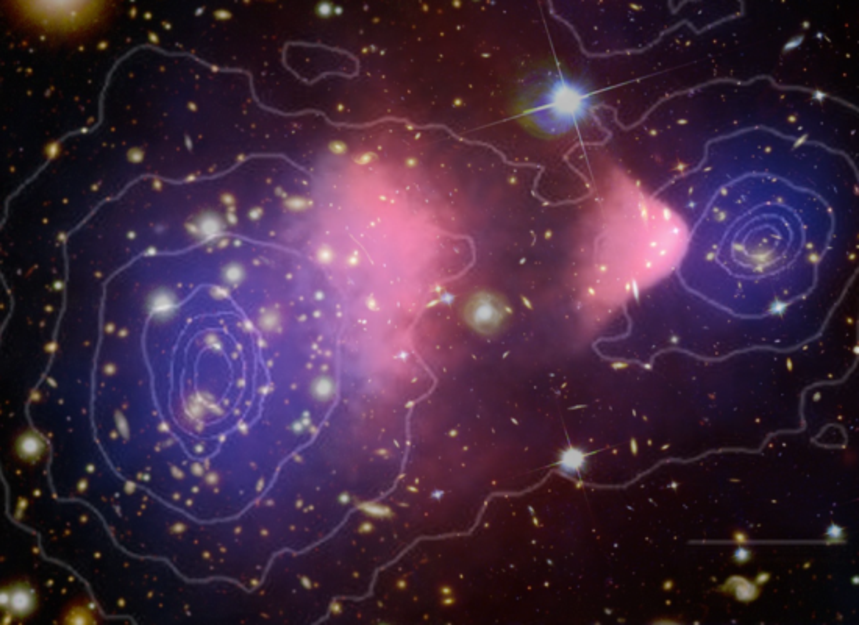
\includegraphics[width = 0.75\textwidth]{img/chapter_1/bullet_cluster.pdf}
    \caption{Image of the Bullet Cluster with contours of the gravitational potential superposed. The red regions indicate the baryonic matter after the collision, while the purple regions are the expected DM components deduced from gravitational lensing. \fixMV{cite}}
    \label{fig:bullet_cluster}
\end{figure}

%%%%%%%%%%%%%%%%%%%%%%%%%%%%%%%%%%%%%
%%%%%%%%%%%%%%%%%%%%%%%%%%%%%%%%%%%%%
\subsection{Cosmological Evidence}
%%%%%%%%%%%%%%%%%%%%%%%%%%%%%%%%%%%%%
%%%%%%%%%%%%%%%%%%%%%%%%%%%%%%%%%%%%%

Dark matter has played a major role in the cosmological history of our universe. The current best cosmological model is the $\Lambda$-Cold Dark Matter model ($\Lambda$CDM), in which cold (i.e. non-relativistic) dark matter plays a prominent role.

\subsubsection*{The Cosmic Microwave Background}
One of the best probes of cosmological models is the Cosmic Microwave Background (CMB). 

\subsubsection*{Big Bang Nucleosynthesis}

\subsubsection*{Large Scale Structure (?)}
The density perturbations in the early universe that would lead to the structures we see today would not have formed without the presence of dark matter. This is due to the pressure on the baryonic matter from the photon gas would have been great enough to prevent the matter from clumping. As dark matter does not significantly (if at all) interact with light, the gravitational pull of the dark matter was able to overcome this pressure.

%%%%%%%%%%%%%%%%%%%%%%%%%%%%%%%%%%%%%
%%%%%%%%%%%%%%%%%%%%%%%%%%%%%%%%%%%%%
%%%%%%%%%%%%%%%%%%%%%%%%%%%%%%%%%%%%%
\section{Potential Models of Dark Matter}
%%%%%%%%%%%%%%%%%%%%%%%%%%%%%%%%%%%%%
%%%%%%%%%%%%%%%%%%%%%%%%%%%%%%%%%%%%%
%%%%%%%%%%%%%%%%%%%%%%%%%%%%%%%%%%%%%

The general consensus amongst physicists is that dark matter has a particle nature, similar to the visible matter of the Standard Model. Given the little details we know about dark matter, an enormous library of models produces a viable candidate. There are, however, several generic properties a good dark matter candidate must satisfy.
\begin{itemize}
    \item neutral under EM
    \item self-interactions
    \item 
\end{itemize}

\commMV{An itemised list of WIMPs, Axions, ultralight, SUSY, ...}

\begin{figure}
    \centering
    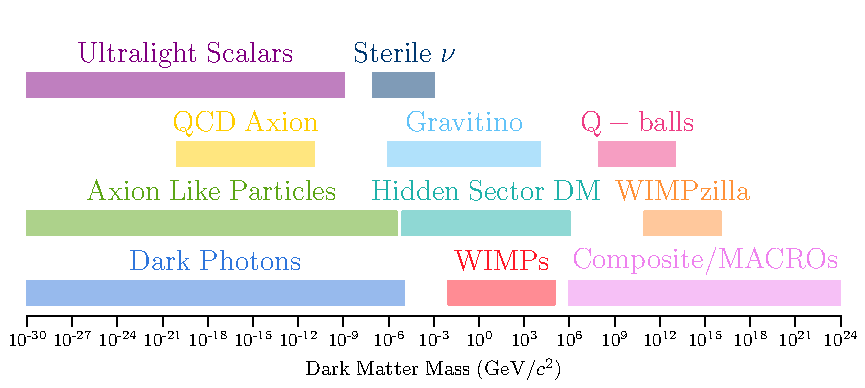
\includegraphics{img/chapter_1/DM_model_landscape.pdf}
    \caption{Illustrative landscape of dark matter models}
    \label{fig:DM_models_landscape}
\end{figure}

%%%%%%%%%%%%%%%%%%%%%%%%%%%%%%%%%%%%%
%%%%%%%%%%%%%%%%%%%%%%%%%%%%%%%%%%%%%
\subsection{Dark Matter in an Effective Fields Theory Framework}
%%%%%%%%%%%%%%%%%%%%%%%%%%%%%%%%%%%%%
%%%%%%%%%%%%%%%%%%%%%%%%%%%%%%%%%%%%%


%%%%%%%%%%%%%%%%%%%%%%%%%%%%%%%%%%%%%
%%%%%%%%%%%%%%%%%%%%%%%%%%%%%%%%%%%%%
%%%%%%%%%%%%%%%%%%%%%%%%%%%%%%%%%%%%%
\section{Current Status of Dark Matter Constraints}
%%%%%%%%%%%%%%%%%%%%%%%%%%%%%%%%%%%%%
%%%%%%%%%%%%%%%%%%%%%%%%%%%%%%%%%%%%%
%%%%%%%%%%%%%%%%%%%%%%%%%%%%%%%%%%%%%

%%%%%%%%%%%%%%%%%%%%%%%%%%%%%%%%%%%%%
%%%%%%%%%%%%%%%%%%%%%%%%%%%%%%%%%%%%%
\subsection{Collider Bounds}
%%%%%%%%%%%%%%%%%%%%%%%%%%%%%%%%%%%%%
%%%%%%%%%%%%%%%%%%%%%%%%%%%%%%%%%%%%%

%%%%%%%%%%%%%%%%%%%%%%%%%%%%%%%%%%%%%
%%%%%%%%%%%%%%%%%%%%%%%%%%%%%%%%%%%%%
\subsection{Direct Detection Searches}
%%%%%%%%%%%%%%%%%%%%%%%%%%%%%%%%%%%%%
%%%%%%%%%%%%%%%%%%%%%%%%%%%%%%%%%%%%%

%%%%%%%%%%%%%%%%%%%%%%%%%%%%%%%%%%%%%
%%%%%%%%%%%%%%%%%%%%%%%%%%%%%%%%%%%%%
\subsection{Indirect Detection}
%%%%%%%%%%%%%%%%%%%%%%%%%%%%%%%%%%%%%
%%%%%%%%%%%%%%%%%%%%%%%%%%%%%%%%%%%%%


It is this route that we will follow to explore dark matter EFTs.

%%%%%%%%%%%%%%%%%%%%%%%%%%%%%%%%%%%%%
%%%%%%%%%%%%%%%%%%%%%%%%%%%%%%%%%%%%%
%%%%%%%%%%%%%%%%%%%%%%%%%%%%%%%%%%%%%
\section{Compact Objects as Dark Matter Probes}
%%%%%%%%%%%%%%%%%%%%%%%%%%%%%%%%%%%%%
%%%%%%%%%%%%%%%%%%%%%%%%%%%%%%%%%%%%%
%%%%%%%%%%%%%%%%%%%%%%%%%%%%%%%%%%%%%


Compact objects, namely Neutron Stars and White Dwarfs, offer a unique
laboratory for studying dark matter interactions. Their extreme environments
offer many benefits in comparison to direct detection experiments. 
These include:

\begin{itemize}
\item \textbf{Gravitational focusing of the DM flux.} In the NS case, the 
infalling DM will be boosted to semi-relativistic velocities ($\sim 0.2 - 0.7 c$
depending on the NS mass).
\item 
\end{itemize}


\begin{figure}
    \centering
    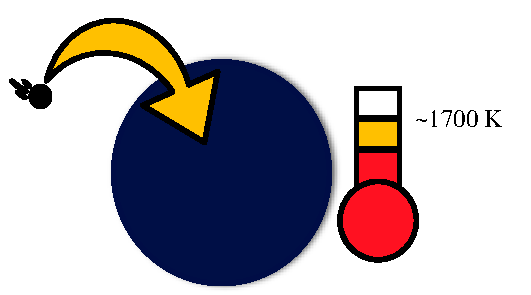
\includegraphics[width=0.45\textwidth]{img/chapter_1/kin_heat_NS.pdf}
    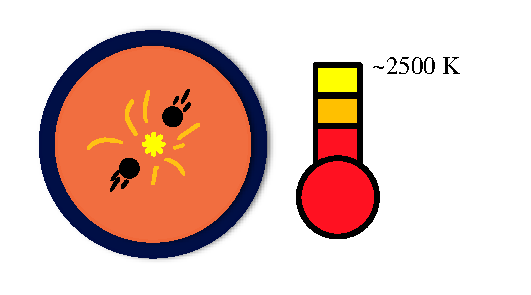
\includegraphics[width=0.45\textwidth]{img/chapter_1/ann_heat_NS.pdf}
    \caption{Illustration of DM-induced heating of compact objects. \textbf{Left:} kinetic heating due to DM scattering, raising the temperature to $\sim 1700 \K$. \textbf{Right:} further annihilation heating adding an additional $\sim 800\K$.}
    \label{fig:cartoon_NS_heat}
\end{figure}




